\chapter{Environment}\label{ch:environment}

This chapter aggregates the previous information and introduces the Reinforcement Learning environment that simulates an initial circular orbit of a satellite in low earth orbit and an accelerated Orbital Decay. The initial conditions, the dynamics of the system, the action and observation space, a distributed optimization of PPO algorithm's hyper-parameter, an evaluation of PPO within this environment, and an analysis of the resulting PPO agent.

\section{Environment Description}

The dynamics of the environment follows that of the physics of Chapter~\ref{ch:physics}. The base of the environment revolves around Algorithm~\ref{alg:problemsim} using the 4th Order Yoshida integrator to calculate the next step's velocity and position from the previous velocity and position and the state's acceleration calculated from the gravitational force and the amplified Drag. 

One aspect of the Environment not yet described in Chapter~\ref{ch:physics} and Section~\ref{sec:reinforcement_learning} is how the satellite agent interacts with it's environment. The maximum force of propulsion of the satellite is a fraction of that of Ion Thruster at $0.04$ Newtons and, it being in a 2D-world or on a plane in a 3D-world, restricting its angle of thrust to a single degree of freedom with values between 0\si{\degree} and 360\si{\degree}. The agent operates in continuous action space with 2 values between 0 and 1. These two input values are not directly map to $[0, 0.04]$ for thrust and $[0, 360)$ as would be natural, but, to reduce variance, it is instead mapped to a delta of the thrust and angle values. This delta's range is $\frac{1}{50}$th the maximum thrust and $\frac{1}{6}$th the maximum angle. If the resulting value of the thrust after applying it's delta is greater than $0.04$ or less than $0$ it is clipped. On the other hand, the angle is wrapped to be between $-\pi$ and $\pi$ after applying the angle delta. The initial thrust is 0 and the initial thrust angle is normal to the origin. The height of the satellite is 550\si{km} from the surface or a radius of $6.921\times 10^6\si{meters}$. The mass of the satellite is 100\si{kg}, 75\si{kg} of which is propellant. Every step in the environment is equivalent to a second. The more massive object, to resemble earth has the same gravitational parameter, $3.986004418\times 10^{14}\si{m^3s^{-2}}$. The surface area of the satellite normal to the velocity is 1\si{m}, this is used while calculating the drag, while the drag coefficient is set to 2.123. As per Chapter~\ref{ch:physics}, the initial orbital velocity is $$v_{\text{orbital}}=\sqrt{\frac{GM}{r}}$$ where $GM$ is the gravitational parameter and $r$ is the radius from our stationary earth located at the origin. The force on the satellite is calculated using equation~\ref{eq:force} with a normal variation of 10\% of the force, but the density, $\rho$ in addition to using equation~\ref{eq:density} to initially calculate, it is multiplied by a hyper-parameter, $\xi$. With the termination threshold for the distance from the target orbit being 1\si{m}, the $\xi$ hyper-parameter is tuned so the density of the atmosphere results in an orbital decay where this termination threshold is reached in 200 steps, if no propulsion is used. The target of this agent in this environment is to maximize the number of steps within the termination threshold while having limited fuel. This means also minimizing the amount of fuel used.

To simplify the calculation of the remaining fuel and mass after each step, the satellite is given enough fuel for 125 steps at maximum thrust. A counter is kept that keeps track of the accumulated thrust before the mapping, which has the range $[0, 1]$. This accumulated thrust is then used to calculate if this threshold has been reached and remaining fuel mass. The mass of the satellite is also adjusted according to the remaining fuel.

The observation space is also continuous of size 8. It includes the normalized position with respect to the initial radius, normalized velocity with respect to the initial velocity, the euclidean distance between the satellite and the target orbit, the euclidean distance between the current velocity and the target velocity for the target circular orbit, the current angle, and the current thrust. All of these values are mapped to be between 0 and 1 before returning to them to the RL algorithm,
$$[r_x, r_y, v_x, v_y, r_{\text{targ}}, v_{\text{targ}}, \theta, F_{\text{thrust}}].$$
Where $r_{targ}=|||\vec{r}||_2 - r_\text{orbital}|$, $v_{\text{targ}}=|||\vec{v}||_2-v_\text{orbital}|$, $||x||_2$ is the euclidean norm operation, $|x|$ is the absolute value operation, $r_\text{orbital}$ is the starting radius, $\vec{r}$ is the current position of the satellite, and $\vec{v}$ is the current velocity of the satellite. The action space, as mentioned before, is continuous, has a size of 2, and includes the thrust delta and the angle delta, $$[\Delta F_{\text{thrust}}, \Delta \theta].$$ 

For every step, the reward signal consists of the current step of the environment divided by 800 plus 0.5 and if the agent either crosses the orbital termination threshold or if it runs out of fuel the episode ends with 0 reward for that step. This linear increase of the reward per step encourages the agent to both not run out of fuel and stay within the orbital termination threshold. $$
r_t = \begin{cases}
	0 & \mbox{if }r_{\text{targ}}>r_{\text{threshold}}\lor f_{\text{used}}>f_{\text{available}} \\
	\frac{t_{\text{step}}}{800} + 0.5 & \mbox{otherwise}
\end{cases}
$$ 
Where $r_{\text{targ}}$ is the distance from the target orbit, $r_{\text{threshold}}$ is the threshold, $f_{\text{used}}$ is the amount of fuel used, $f_{\text{available}}$ is the amount of fuel available, and $t_{\text{step}}$ is the number of steps since the start of the episode. If the environment's episode reaches 800 steps it is ended.

\begin{figure}
	\centering
	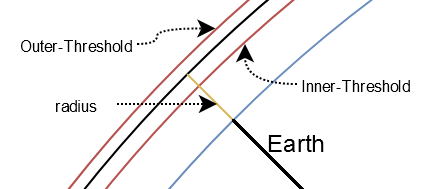
\includegraphics{OrbitDiagram}
	\caption{A diagram of the target orbit and the termination orbital threshold.}
	\label{fig:OrbitDiagram}
\end{figure}

Normally calculating the acceleration, the velocity and position using the 4th order yoshida integrator is computationally expensive, especially because the language, python, used is not a compiled language. This is mitigated using the Numba \cite{10.1145/2833157.2833162} library. Using Numba, the portion of the code that calculates the acceleration and calculates the 4th order yoshida integration are compiled to binary using a Just-in-time (JIT) compiler.
	
\section{Distributed Hyper-parameter Optimization}

\section{Training \& Evaluation}

\section{Discussion}